% Options for packages loaded elsewhere
\PassOptionsToPackage{unicode}{hyperref}
\PassOptionsToPackage{hyphens}{url}
%
\documentclass[
]{article}
\usepackage{amsmath,amssymb}
\usepackage{lmodern}
\usepackage{iftex}
\ifPDFTeX
  \usepackage[T1]{fontenc}
  \usepackage[utf8]{inputenc}
  \usepackage{textcomp} % provide euro and other symbols
\else % if luatex or xetex
  \usepackage{unicode-math}
  \defaultfontfeatures{Scale=MatchLowercase}
  \defaultfontfeatures[\rmfamily]{Ligatures=TeX,Scale=1}
\fi
% Use upquote if available, for straight quotes in verbatim environments
\IfFileExists{upquote.sty}{\usepackage{upquote}}{}
\IfFileExists{microtype.sty}{% use microtype if available
  \usepackage[]{microtype}
  \UseMicrotypeSet[protrusion]{basicmath} % disable protrusion for tt fonts
}{}
\makeatletter
\@ifundefined{KOMAClassName}{% if non-KOMA class
  \IfFileExists{parskip.sty}{%
    \usepackage{parskip}
  }{% else
    \setlength{\parindent}{0pt}
    \setlength{\parskip}{6pt plus 2pt minus 1pt}}
}{% if KOMA class
  \KOMAoptions{parskip=half}}
\makeatother
\usepackage{xcolor}
\usepackage[margin=1in]{geometry}
\usepackage{graphicx}
\makeatletter
\def\maxwidth{\ifdim\Gin@nat@width>\linewidth\linewidth\else\Gin@nat@width\fi}
\def\maxheight{\ifdim\Gin@nat@height>\textheight\textheight\else\Gin@nat@height\fi}
\makeatother
% Scale images if necessary, so that they will not overflow the page
% margins by default, and it is still possible to overwrite the defaults
% using explicit options in \includegraphics[width, height, ...]{}
\setkeys{Gin}{width=\maxwidth,height=\maxheight,keepaspectratio}
% Set default figure placement to htbp
\makeatletter
\def\fps@figure{htbp}
\makeatother
\setlength{\emergencystretch}{3em} % prevent overfull lines
\providecommand{\tightlist}{%
  \setlength{\itemsep}{0pt}\setlength{\parskip}{0pt}}
\setcounter{secnumdepth}{5}
\ifLuaTeX
  \usepackage{selnolig}  % disable illegal ligatures
\fi
\IfFileExists{bookmark.sty}{\usepackage{bookmark}}{\usepackage{hyperref}}
\IfFileExists{xurl.sty}{\usepackage{xurl}}{} % add URL line breaks if available
\urlstyle{same} % disable monospaced font for URLs
\hypersetup{
  pdftitle={upf salt content},
  pdfauthor={doh},
  hidelinks,
  pdfcreator={LaTeX via pandoc}}

\title{upf salt content}
\author{doh}
\date{2023-02-16}

\begin{document}
\maketitle

{
\setcounter{tocdepth}{2}
\tableofcontents
}
\hypertarget{nutrient-database-proportions-of-foods-which-are-upf-nova-4}{%
\subsection{Nutrient database proportions of foods which are UPF (NOVA
4)}\label{nutrient-database-proportions-of-foods-which-are-upf-nova-4}}

This script will use UPFNOVA to identify foods within the database which
are UPF. Comparison can then be made between 2008 and 2019.

\begin{verbatim}
## 
## Attaching package: 'dplyr'
\end{verbatim}

\begin{verbatim}
## The following objects are masked from 'package:data.table':
## 
##     between, first, last
\end{verbatim}

\begin{verbatim}
## The following objects are masked from 'package:stats':
## 
##     filter, lag
\end{verbatim}

\begin{verbatim}
## The following objects are masked from 'package:base':
## 
##     intersect, setdiff, setequal, union
\end{verbatim}

\hypertarget{including-plots}{%
\subsection{Including Plots}\label{including-plots}}

You can also embed plots, for example:

\begin{verbatim}
##                                                 food name food group number
##   1:                                                Pizza                1C
##   2:         Pasta (manufactured products and ready meals                1D
##   3:             Pasta (other, including homemade dishes)                1E
##   4:         Rice (manufactured products and ready meals)                1F
##   5:              Rice (other, including homemade dishes)                1G
##  ---                                                                       
## 151:             58B Soft drinks low calorie carbonated 4               58B
## 152: 58C Soft drinks low calorie, ready to drink, still 4               58C
## 153:            59R Brown, granary and wheat germ bread 4               59R
## 154:                                        60R 1% Milk 1               60R
## 155:                                      61R Smoothies 1               61R
##      Nova group
##   1:          4
##   2:          4
##   3:          n
##   4:          4
##   5:          n
##  ---           
## 151:          4
## 152:          4
## 153:          4
## 154:          1
## 155:          1
\end{verbatim}

\begin{verbatim}
## Null data.table (0 rows and 0 cols)
\end{verbatim}

\hypertarget{does-nova-group-predict-the-salt-content}{%
\subsubsection{Does Nova group predict the salt
content?}\label{does-nova-group-predict-the-salt-content}}

first in year 1 2008

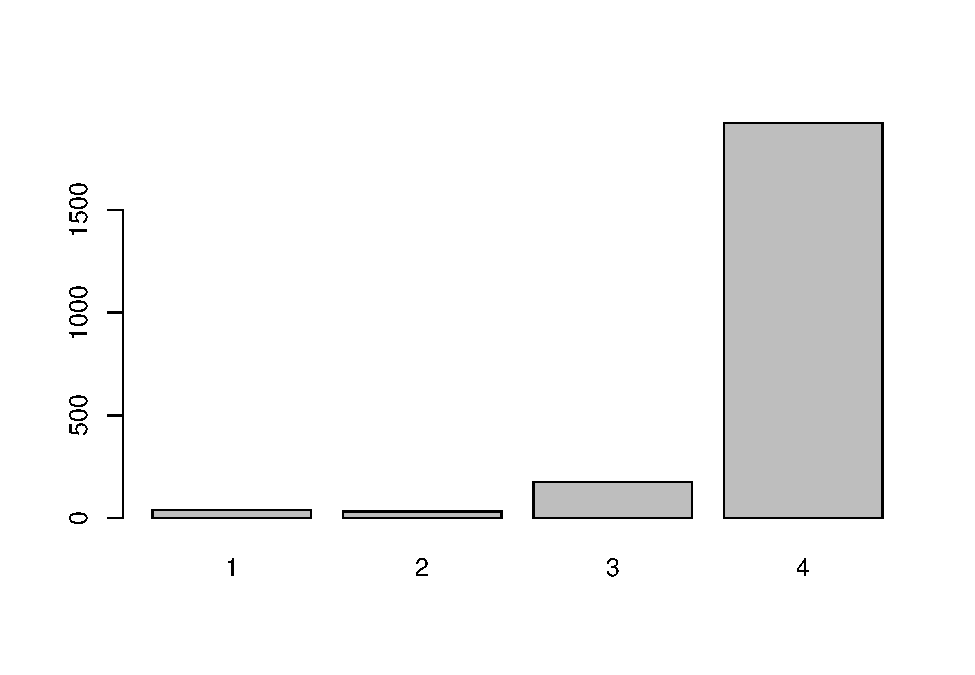
\includegraphics{upfsnutrient_files/figure-latex/unnamed-chunk-2-1.pdf}
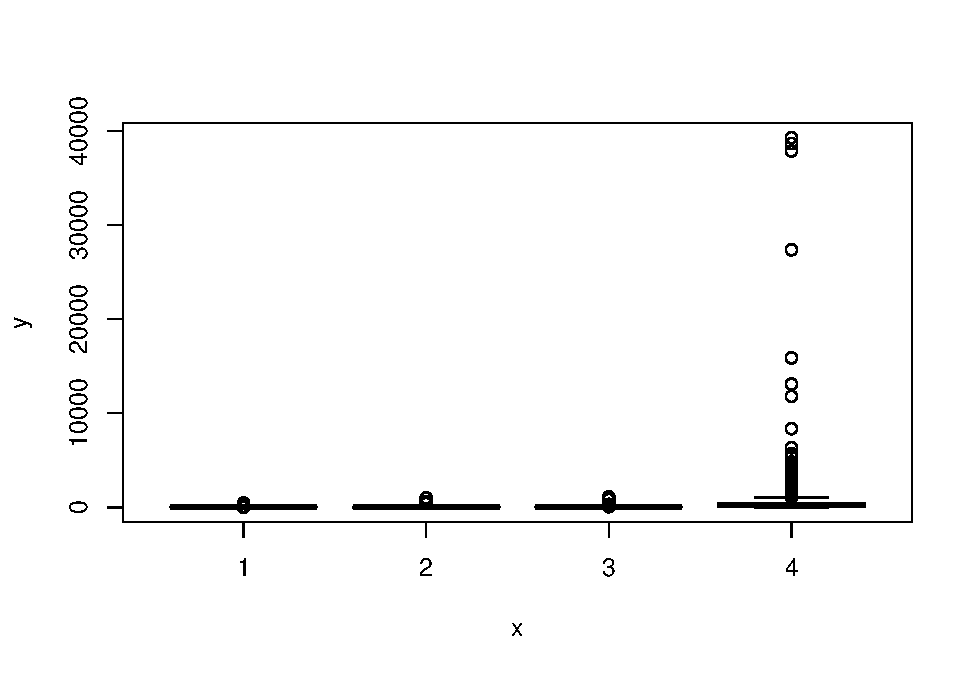
\includegraphics{upfsnutrient_files/figure-latex/unnamed-chunk-2-2.pdf}
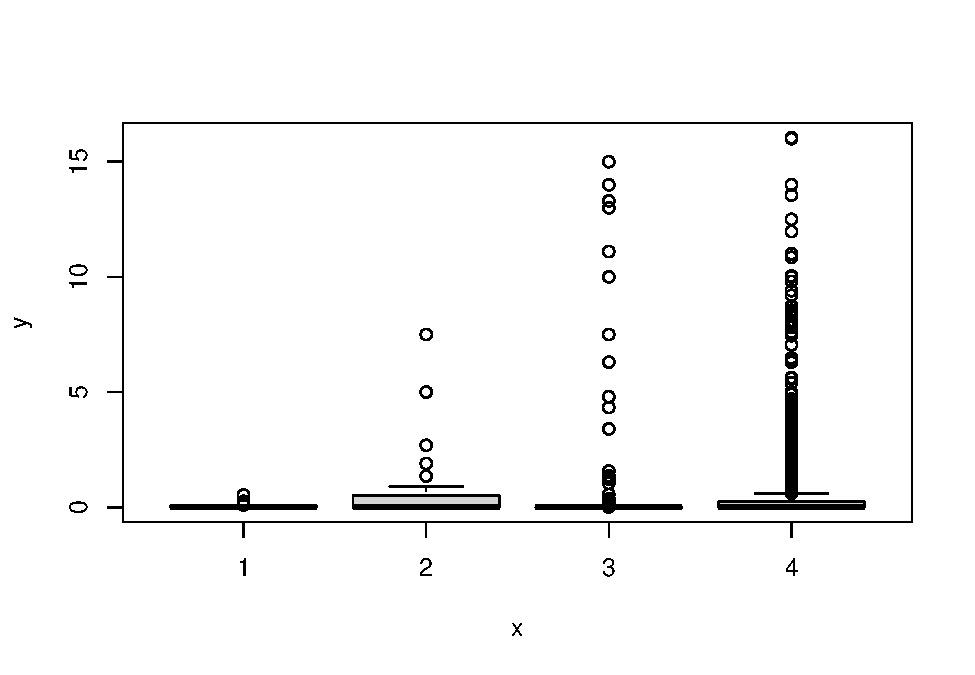
\includegraphics{upfsnutrient_files/figure-latex/unnamed-chunk-2-3.pdf}

\begin{verbatim}
## 
## Call:
## lm(formula = Sodium ~ `Nova group`, data = nasubset)
## 
## Coefficients:
##   (Intercept)  `Nova group`2  `Nova group`3  `Nova group`4  
##        51.289         58.992         -7.455        407.179
\end{verbatim}

then in year 11 2019

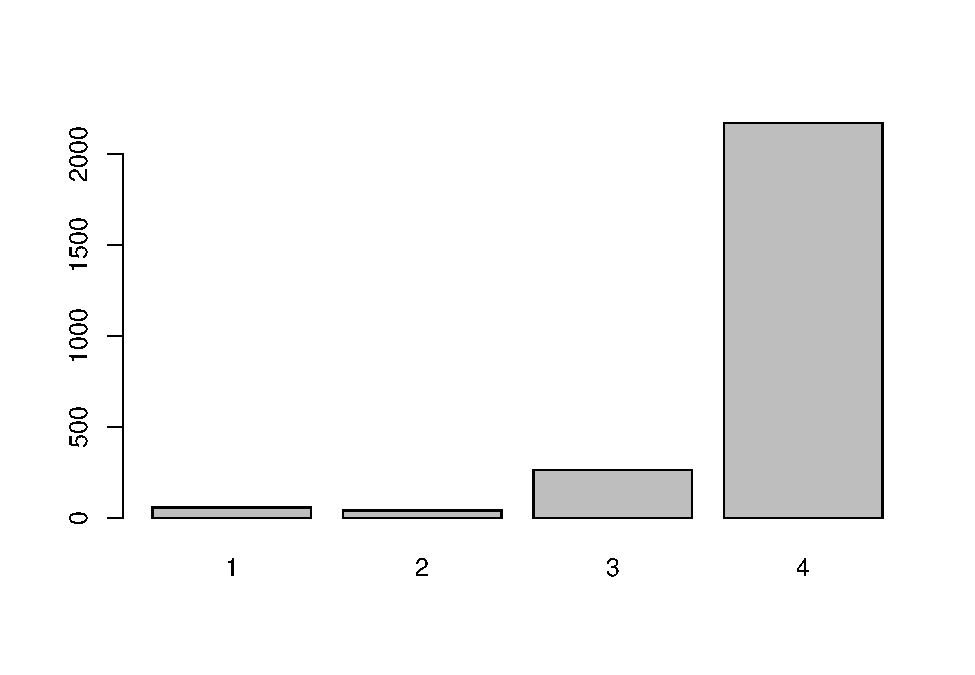
\includegraphics{upfsnutrient_files/figure-latex/unnamed-chunk-3-1.pdf}

\begin{verbatim}
## 
## Call:
## lm(formula = Sodium ~ `Nova group`, data = nasubset)
## 
## Coefficients:
##   (Intercept)  `Nova group`2  `Nova group`3  `Nova group`4  
##         39.36          53.91          32.47         361.93
\end{verbatim}

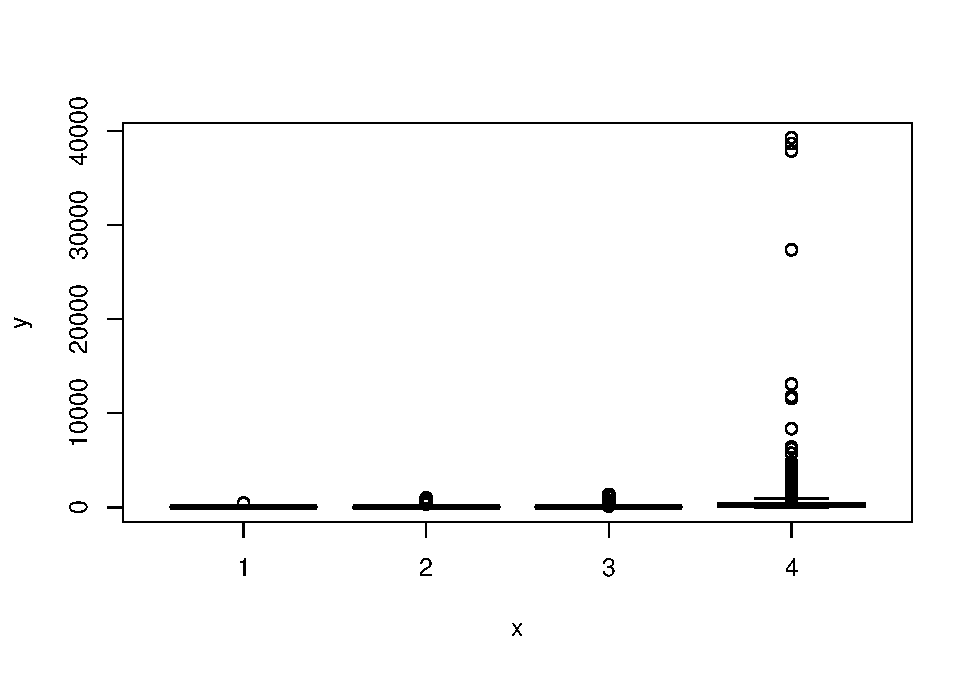
\includegraphics{upfsnutrient_files/figure-latex/unnamed-chunk-3-2.pdf}
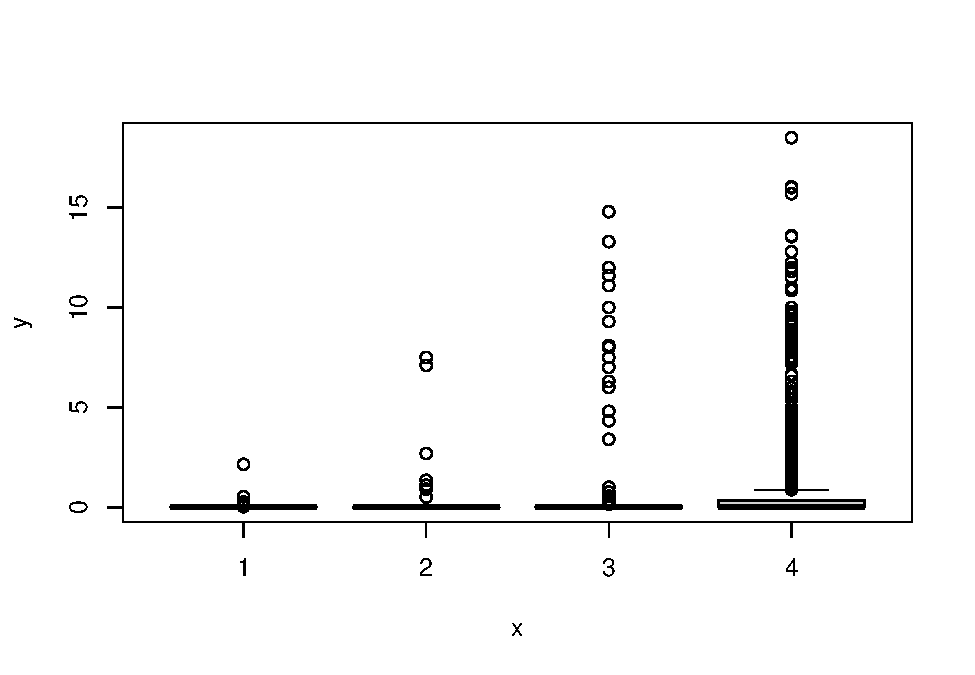
\includegraphics{upfsnutrient_files/figure-latex/unnamed-chunk-3-3.pdf}

Nova group 4 still is much more likely to contain sodium.

\end{document}
